想象你是一位工程师，被要求从零开始设计一台计算机. 有一天你正在办公室里埋头工作，设计逻辑电路，布置 \texttt{AND} 门、\texttt{OR} 门等等，这时你的老板走进来带来了坏消息. 客户刚刚增加了一项令人惊讶的设计要求：整台计算机的电路只能有两层：

\begin{center}
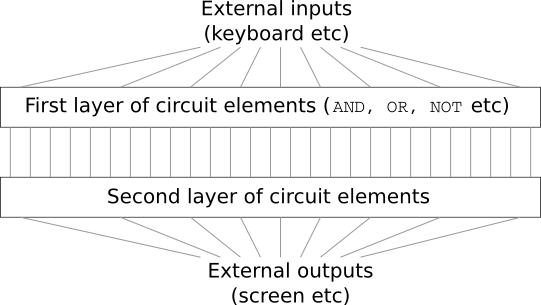
\includegraphics[width=0.833\textwidth]{images/shallow_circuit.png}
\end{center}

\noindent 你目瞪口呆，对老板说：``客户疯了！''

你的老板回答：``我也觉得他们疯了. 但客户想要什么，就得给他们什么.''

事实上，在有限的意义上，客户并没有疯. 假设你可以使用一种特殊的逻辑门，它允许你把任意多个输入 \texttt{AND} 在一起. 而且你还可以使用一个多输入 \texttt{NAND} 门，也就是说，一个可以将多个输入 \texttt{AND} 起来然后对输出取反的门. 有了这些特殊的门，事实证明可以用一个仅两层的电路来计算任意函数.

但仅仅因为某件事是可能的，并不意味着它是一个好主意. 在实践中，当解决电路设计问题（或几乎任何类型的算法问题）时，我们通常先弄清楚如何解决子问题，然后逐步整合这些解决方案. 换句话说，我们通过多层抽象来构建解决方案.

例如，假设我们正在设计一个逻辑电路来将两个数相乘. 很可能我们希望用执行两个数相加等操作的子电路来构建它. 用于两个数相加的子电路，又会由用于两个比特相加的子子电路构建而成. 粗略地说，我们的电路看起来像这样：

\begin{center}
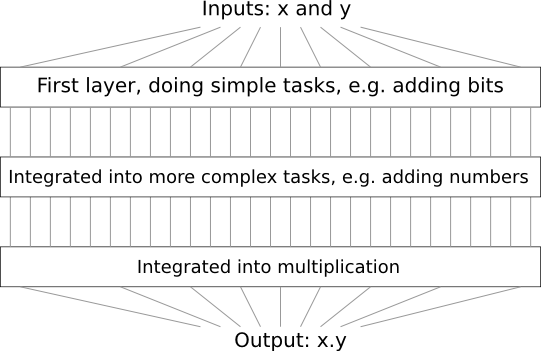
\includegraphics[width=0.833\textwidth]{images/circuit_multiplication.png}
\end{center}

\noindent 也就是说，我们最终的电路至少包含三层电路元件. 事实上，它很可能包含超过三层，因为我们会把子任务分解成比我描述的更小的单元. 但你明白大意了.

所以深层电路使设计过程更容易. 但它们不仅仅对设计有帮助. 事实上，有数学证明表明，对于某些函数，非常浅的电路需要指数级更多的电路元件才能计算，而深层电路则不需要. 例如，20 世纪 80 年代初一系列著名的论文*\footnote{这段历史有些复杂，所以我不会给出详细的参考文献. 参见 Johan Håstad 2012 年的论文 On the correlation of parity and small-depth circuits，其中有早期历史的叙述和参考文献.}表明，如果用浅层电路来计算一组比特的奇偶性，需要指数级多的门. 另一方面，如果你使用更深的电路，用一个小电路就可以轻松计算奇偶性：你只需计算每对比特的奇偶性，然后用这些结果计算每对比特对的奇偶性，依此类推，很快就能构建出整体的奇偶性. 因此，深层电路本质上可以比浅层电路强大得多.

到目前为止，本书对待神经网络的方式就像那个疯狂的客户一样. 我们使用过的几乎所有网络都只有一个隐藏神经元层（加上输入层和输出层）：

\begin{center}
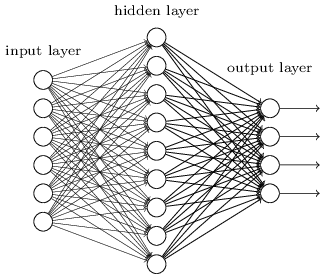
\includegraphics[width=0.9\textwidth]{images/tikz35.png}
\end{center}

\noindent 这些简单的网络非常有用：在前面的章节中，我们用这样的网络对手写数字进行分类，准确率超过了 98\%！尽管如此，直觉上我们会期望具有更多隐藏层的网络更加强大：

\begin{center}
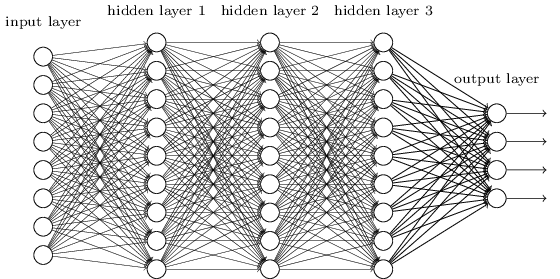
\includegraphics[width=0.9\textwidth]{images/tikz36.png}
\end{center}

\noindent 这样的网络可以利用中间层来构建多层抽象，就像我们在布尔电路中所做的那样. 例如，如果我们正在进行视觉模式识别，那么第一层的神经元可能学会识别边缘，第二层的神经元可以学会识别更复杂的形状，比如由边缘构成的三角形或矩形. 第三层则会识别更加复杂的形状. 依此类推. 这些多层抽象似乎很可能赋予深层网络在学习解决复杂模式识别问题方面的显著优势. 此外，正如电路的情况一样，有理论结果表明深层网络本质上比浅层网络更加强大*\footnote{对于某些问题和网络架构，这一点在 On the number of response regions of deep feed forward networks with piece-wise linear activations 中得到了证明，作者是 Razvan Pascanu、Guido Montúfar 和 Yoshua Bengio（2014）. 另见 Yoshua Bengio（2009）的 Learning deep architectures for AI 第 2 节中更非正式的讨论.}.

我们如何训练这样的深层网络呢？在本章中，我们将尝试使用我们的主力学习算法——通过反向传播的随机梯度下降——来训练深层网络. 但我们会遇到麻烦，我们的深层网络表现并不比浅层网络好多少（如果有的话）.

鉴于上面的讨论，这种失败似乎令人惊讶. 我们不会放弃深层网络，而是要深入挖掘，试图理解是什么让我们的深层网络难以训练. 当我们仔细观察时，我们会发现深层网络中不同的层以极其不同的速度学习. 特别是，当网络中较后的层学习得很好时，较早的层在训练过程中常常陷入停滞，几乎学不到任何东西. 这种停滞不仅仅是运气不好. 相反，我们会发现学习放缓的发生有根本性的原因，与我们使用基于梯度的学习技术有关.

当我们更深入地探究这个问题时，我们会了解到相反的现象也可能发生：较早的层可能学习得很好，但较后的层可能陷入停滞. 事实上，我们会发现，在深层的多层神经网络中，通过梯度下降进行学习存在一种内在的不稳定性. 这种不稳定性往往导致较早或较后的层在训练过程中陷入停滞.

这一切听起来像是坏消息. 但通过深入研究这些困难，我们可以开始洞察有效训练深层网络所需的条件. 因此这些研究为下一章做了很好的准备，在下一章中我们将使用深度学习来攻克图像识别问题.
\sectionTitle{梯度消失问题}{梯度消失问题}

那么，当我们尝试训练一个深度网络时，究竟出了什么问题？

为了回答这个问题，让我们首先回顾一下只有一个隐藏层的网络的情况. 像往常一样，我们将使用 MNIST 数字分类问题作为学习和实验的游乐场*\footnote{我在这里和这里介绍了 MNIST 问题和数据.}.

如果你愿意，你可以在自己的计算机上训练网络来跟随学习. 当然，仅仅阅读也是可以的. 如果你确实想实时跟随，那么你需要 Python 2.7、Numpy 以及一份代码，你可以通过从命令行克隆相关仓库来获取：

\begin{lstlisting}
git clone https://github.com/mnielsen/neural-networks-and-deep-learning.git

\end{lstlisting}

如果你不使用 git，那么你可以在这里下载数据和代码. 你需要切换到 src 子目录.

然后，从 Python shell 中加载 MNIST 数据：

\begin{lstlisting}
>>> import mnist_loader
>>> training_data, validation_data, test_data = \
... mnist_loader.load_data_wrapper()

\end{lstlisting}

我们建立网络：

\begin{lstlisting}
>>> import network2
>>> net = network2.Network([784, 30, 10])

\end{lstlisting}

这个网络在输入层有 784 个神经元，对应于输入图像中的 $28 \times 28 = 784$ 个像素. 我们使用 30 个隐藏神经元，以及 10 个输出神经元，对应于 MNIST 数字的 10 种可能分类（'0'、'1'、'2'、$\ldots$、'9'）.

让我们尝试用 30 个完整的轮次来训练我们的网络，每次使用 10 个训练样本的小批量，学习率 $\eta = 0.1$，正则化参数 $\lambda = 5.0$. 在训练过程中，我们将监控 \texttt{validation\_\allowbreak{}data} 上的分类准确率*\footnote{请注意，根据你机器的速度，网络训练可能需要几分钟. 因此，如果你正在运行代码，你可能希望继续阅读并稍后回来，而不是等待代码执行完毕.}：

\begin{lstlisting}
>>> net.SGD(training_data, 30, 10, 0.1, lmbda=5.0,
... evaluation_data=validation_data, monitor_evaluation_accuracy=True)

\end{lstlisting}

我们得到了 96.48\% 的分类准确率（或大致如此——每次运行会略有不同），与我们之前使用类似配置得到的结果相当.

现在，让我们再添加一个隐藏层，同样包含 30 个神经元，并尝试使用相同的超参数进行训练：

\begin{lstlisting}
>>> net = network2.Network([784, 30, 30, 10])
>>> net.SGD(training_data, 30, 10, 0.1, lmbda=5.0,
... evaluation_data=validation_data, monitor_evaluation_accuracy=True)

\end{lstlisting}

这给出了一个改进的分类准确率，96.90\%. 这令人鼓舞：稍微增加一点深度是有帮助的. 让我们再添加一个 30 个神经元的隐藏层：

\begin{lstlisting}
>>> net = network2.Network([784, 30, 30, 30, 10])
>>> net.SGD(training_data, 30, 10, 0.1, lmbda=5.0,
... evaluation_data=validation_data, monitor_evaluation_accuracy=True)

\end{lstlisting}

这完全没有帮助. 事实上，结果回落到了 96.57\%，接近我们最初的浅层网络. 假设我们再插入一个隐藏层：

\begin{lstlisting}
>>> net = network2.Network([784, 30, 30, 30, 30, 10])
>>> net.SGD(training_data, 30, 10, 0.1, lmbda=5.0,
... evaluation_data=validation_data, monitor_evaluation_accuracy=True)

\end{lstlisting}

分类准确率再次下降，降至 96.53\%. 这可能不是一个统计上显著的下降，但也不令人鼓舞.

这种行为似乎很奇怪. 直观上，额外的隐藏层应该使网络能够学习更复杂的分类函数，从而更好地进行分类. 当然，情况不应该变得更糟，因为额外的层在最坏的情况下可以简单地什么都不做*\footnote{参见后面的这个习题，了解如何构建一个什么都不做的隐藏层.}. 但事实并非如此.

那么到底发生了什么？让我们假设额外的隐藏层原则上确实可能有帮助，问题在于我们的学习算法没有找到正确的权重和偏置. 我们想弄清楚我们的学习算法出了什么问题，以及如何做得更好.

为了对问题所在有所了解，让我们可视化网络是如何学习的. 下面，我绘制了一个 $[784, 30, 30, 10]$ 网络的一部分，即一个有两个隐藏层的网络，每个隐藏层包含 $30$ 个隐藏神经元. 图中的每个神经元上都有一个小条，表示该神经元在网络学习过程中变化的速度. 大条意味着该神经元的权重和偏置变化很快，而小条意味着权重和偏置变化缓慢. 更精确地说，这些条表示每个神经元的梯度 $\partial C / \partial b$，即代价相对于神经元偏置的变化率. 在第 2 章中我们看到，这个梯度量不仅控制了学习过程中偏置变化的速度，也控制了输入到该神经元的权重变化的速度. 如果你不记得细节，不用担心：需要记住的只是，这些条显示了每个神经元的权重和偏置在网络学习过程中变化的速度.

为了保持图简单，我只展示了两个隐藏层中前六个神经元. 我省略了输入神经元，因为它们没有需要学习的权重或偏置. 我也省略了输出神经元，因为我们正在进行逐层比较，而比较具有相同神经元数量的层最有意义. 结果绘制在训练的最开始，即网络初始化之后立即. 它们在这里*\footnote{绘制的数据是使用程序 generate\_\allowbreak{}gradient.py 生成的. 同一程序也用于生成本节后面引用的结果.}：网络是随机初始化的，因此神经元学习速度存在很大差异并不奇怪. 尽管如此，引人注目的是第二个隐藏层中的条大多比第一个隐藏层中的条大得多. 因此，第二个隐藏层中的神经元将比第一个隐藏层中的神经元学习得快得多. 这仅仅是巧合，还是第二个隐藏层中的神经元通常可能比第一个隐藏层中的神经元学习得更快？

为了确定是否如此，有一种全局的方法来比较第一和第二隐藏层的学习速度会很有帮助. 为此，让我们将梯度记为 $\delta^l_j = \partial C / \partial b^l_j$，即第 $l$ 层中第 $j$ 个神经元的梯度*\footnote{在第 2 章中我们将其称为误差，但这里我们将采用非正式的术语``梯度''. 我说``非正式''是因为这当然没有明确包括代价相对于权重的偏导数 $\partial C / \partial w$.}. 我们可以将梯度 $\delta^1$ 视为一个向量，其元素决定了第一个隐藏层学习的速度，而 $\delta^2$ 视为一个向量，其元素决定了第二个隐藏层学习的速度. 然后我们将使用这些向量的长度作为各层学习速度的（粗略的！）全局度量. 例如，长度 $\| \delta^1 \|$ 衡量第一个隐藏层学习的速度，而长度 $\| \delta^2 \|$ 衡量第二个隐藏层学习的速度.

有了这些定义，在与上面绘制的相同配置中，我们发现 $\| \delta^1 \| = 0.07\ldots$ 和 $\| \delta^2 \| = 0.31\ldots$. 因此这证实了我们之前的怀疑：第二个隐藏层中的神经元确实比第一个隐藏层中的神经元学习得快得多.

如果我们添加更多的隐藏层会发生什么？如果我们有三个隐藏层，在一个 $[784, 30, 30, 30, 10]$ 网络中，那么各自的学习速度结果是 0.012、0.060 和 0.283. 同样，较早的隐藏层比较晚的隐藏层学习得慢得多. 假设我们再添加一个包含 $30$ 个隐藏神经元的层. 在这种情况下，各自的学习速度是 0.003、0.017、0.070 和 0.285. 模式保持不变：较早的层比较晚的层学习得慢.

我们一直在观察训练开始时的学习速度，即网络初始化之后立即. 随着我们训练网络，学习速度如何变化？让我们回到只有两个隐藏层的网络. 学习速度变化如下：

\begin{center}
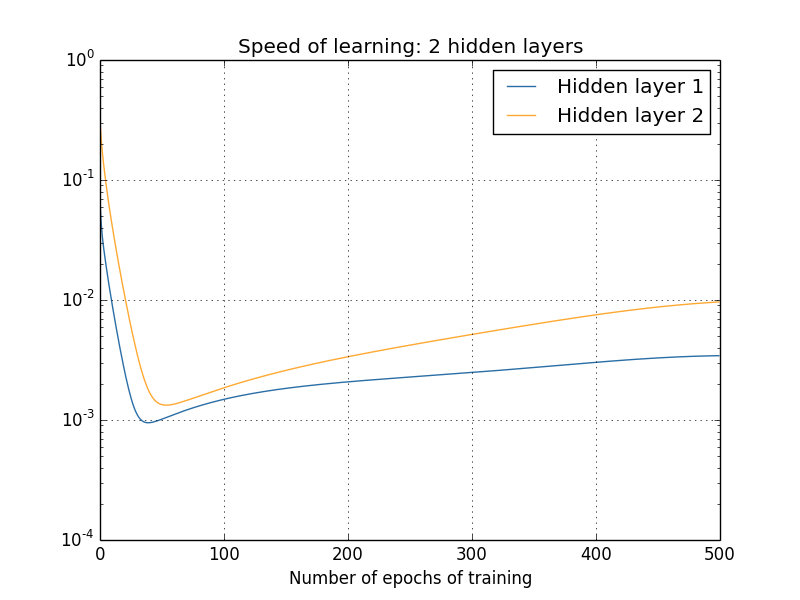
\includegraphics[width=0.833\textwidth]{images/training_speed_2_layers.png}
\end{center}

\noindent 为了生成这些结果，我使用了批量梯度下降，仅用 1,000 张训练图像，训练了 500 个轮次. 这与我们通常的训练方式有些不同——我没有使用小批量，只用了 1,000 张训练图像，而不是完整的 50,000 张图像训练集. 我不是想做什么偷偷摸摸的事，或者蒙蔽你的眼睛，但事实证明，使用小批量随机梯度下降会得到噪声大得多的结果（尽管当你平均掉噪声后，结果非常相似）. 使用我选择的参数是一种平滑结果的简单方法，这样我们就可以看到发生了什么.

无论如何，如你所见，两层一开始的学习速度非常不同（正如我们已经知道的）. 两层的速度随后都迅速下降，然后反弹. 但贯穿始终，第一个隐藏层比第二个隐藏层学习得慢得多.

更复杂的网络呢？这里是一个类似实验的结果，但这次有三个隐藏层（一个 $[784, 30, 30, 30, 10]$ 网络）：

\begin{center}
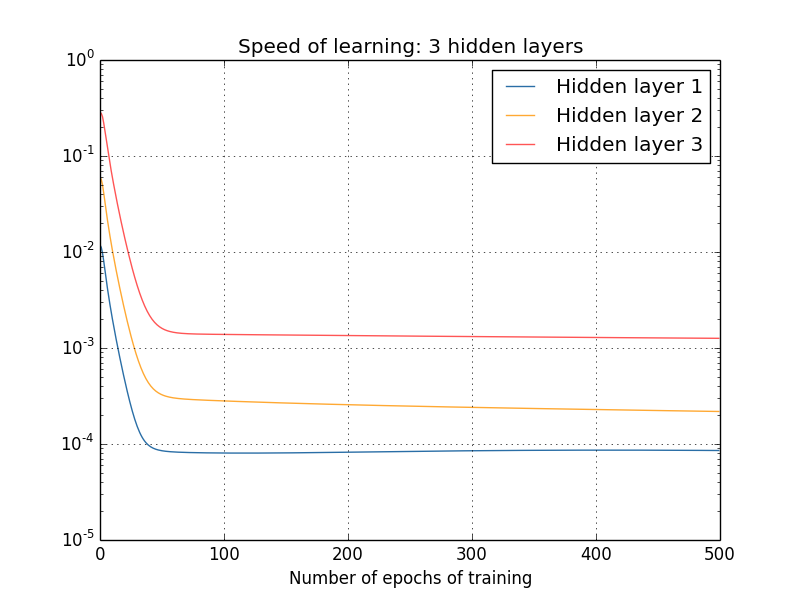
\includegraphics[width=0.833\textwidth]{images/training_speed_3_layers.png}
\end{center}

\noindent 同样，较早的隐藏层比较晚的隐藏层学习得慢得多. 最后，让我们添加第四个隐藏层（一个 $[784, 30, 30, 30, 30, 10]$ 网络），看看训练时会发生什么：

\begin{center}
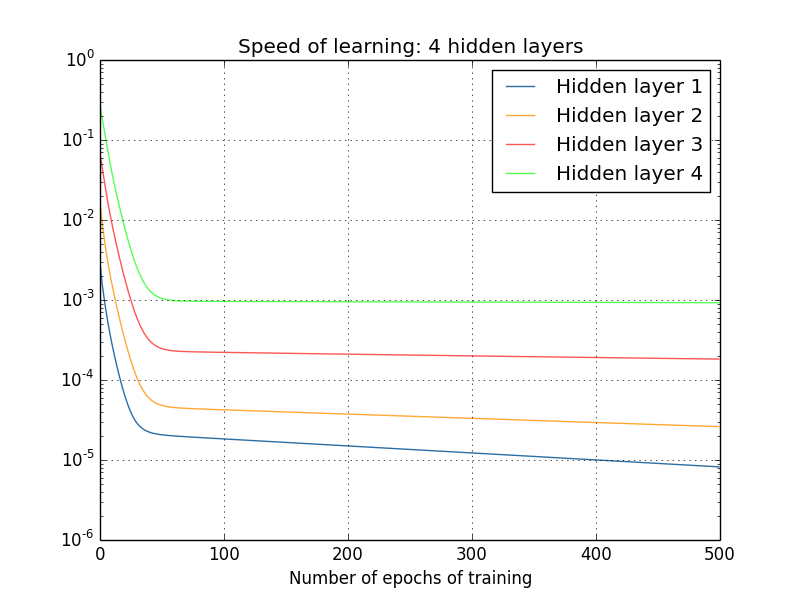
\includegraphics[width=0.833\textwidth]{images/training_speed_4_layers.png}
\end{center}

\noindent 同样，较早的隐藏层比较晚的隐藏层学习得慢得多. 在这种情况下，第一个隐藏层的学习速度大约比最后一个隐藏层慢 100 倍. 难怪我们之前训练这些网络时遇到了麻烦！

我们在这里有一个重要的观察：至少在一些深度神经网络中，梯度随着我们向后穿过隐藏层而趋于变小. 这意味着较早层中的神经元比较晚层中的神经元学习得慢得多. 虽然我们只是在一个网络中看到了这一点，但在许多神经网络中，这种情况的发生有根本原因. 这种现象被称为\emph{梯度消失问题}（vanishing gradient problem）\label{term:63}*\footnote{参见 Gradient flow in recurrent nets: the difficulty of learning long-term dependencies，作者 Sepp Hochreiter、Yoshua Bengio、Paolo Frasconi 和 Jürgen Schmidhuber（2001）. 这篇论文研究的是循环神经网络，但基本现象与我们正在研究的前馈网络相同. 另见 Sepp Hochreiter 早期的文凭论文，Untersuchungen zu dynamischen neuronalen Netzen（1991，德文）.}.

为什么会发生梯度消失问题？有没有办法避免它？在训练深度神经网络时，我们应该如何处理它？事实上，我们很快就会了解到，这并非不可避免，尽管替代方案也不太吸引人：有时梯度在较早的层中变得大得多！这就是\emph{梯度爆炸问题}（exploding gradient problem）\label{term:64}，它并不比梯度消失问题好多少. 更一般地说，事实证明深度神经网络中的梯度是\emph{不稳定的}，在较早的层中倾向于要么爆炸要么消失. 这种不稳定性是深度神经网络中基于梯度的学习的一个根本问题. 这是我们需要理解的，如果可能的话，需要采取措施解决的问题.

对梯度消失（或不稳定）的一种回应是怀疑它们是否真的是一个大问题. 暂时离开神经网络，想象我们试图数值最小化一个单变量函数 $f(x)$. 如果导数 $f'(x)$ 很小，难道不是好消息吗？难道不意味着我们已经接近极值点了吗？类似地，深度网络早期层中的小梯度是否可能意味着我们不需要对权重和偏置做太多调整？

当然，事实并非如此. 回想一下，我们随机初始化了网络中的权重和偏置. 我们初始的权重和偏置极不可能在我们希望网络做的任何事情上表现良好. 具体来说，考虑一个用于 MNIST 问题的 $[784, 30, 30, 30, 10]$ 网络中的第一层权重. 随机初始化意味着第一层丢弃了关于输入图像的大部分信息. 即使后面的层已经经过了广泛的训练，它们仍然会发现识别输入图像极其困难，仅仅因为它们没有足够的信息. 因此，第一层不需要做太多学习的情况不可能成立. 如果我们要训练深度网络，我们需要弄清楚如何解决梯度消失问题.
\sectionTitle{是什么导致了梯度消失问题？深度神经网络中不稳定的梯度}{是什么导致了梯度消失问题？深度神经网络中不稳定的梯度}

为了深入理解梯度消失问题为何会发生，让我们考虑最简单的深度神经网络：每一层只有一个神经元. 下面是一个有三个隐藏层的网络：

\begin{center}
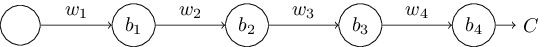
\includegraphics[width=0.9\textwidth]{images/tikz37.png}
\end{center}

\noindent 这里，$w_1, w_2, \ldots$ 是权重，$b_1, b_2, \ldots$ 是偏置，$C$ 是某个代价函数. 为了提醒你它的工作原理，第 $j$ 个神经元的输出 $a_j$ 是 $\sigma(z_j)$，其中 $\sigma$ 是通常的 S 型激活函数，而 $z_j = w_{j} a_{j-1}+b_j$ 是该神经元的加权输入. 我在最后画出了代价 $C$，以强调代价是网络输出 $a_4$ 的函数：如果网络的实际输出接近期望输出，那么代价就低，而如果相差很远，代价就高.

我们将研究第一个隐藏神经元对应的梯度 $\partial C / \partial b_1$. 我们会推导出 $\partial C / \partial b_1$ 的表达式，并通过研究该表达式来理解梯度消失问题为何会发生.

我先直接给你展示 $\partial C / \partial b_1$ 的表达式. 它看起来令人生畏，但实际上有一个简单的结构，我稍后会描述. 下面是这个表达式（暂时忽略网络，注意 $\sigma'$ 只是 $\sigma$ 函数的导数）：

\begin{center}
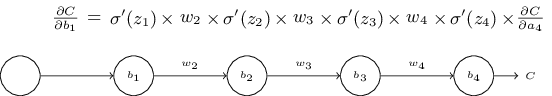
\includegraphics[width=0.9\textwidth]{images/tikz38.png}
\end{center}

\noindent 该表达式的结构如下：网络中每个神经元对应一个 $\sigma'(z_j)$ 项；网络中每个权重对应一个权重 $w_j$ 项；最后还有一个 $\partial C / \partial a_4$ 项，对应于末端的代价函数. 注意我把每一项都放在了网络中对应部分的上方. 因此，网络本身就是该表达式的一个助记符.

你可以直接接受这个表达式，跳到关于它与梯度消失问题关系的讨论. 这样做没有坏处，因为该表达式是我们之前讨论的反向传播的一个特例. 但关于这个表达式为何成立也有一个简单的解释，所以看一看那个解释是很有趣的（也许还有启发意义）.

想象我们对偏置 $b_1$ 做一个微小的改变 $\Delta b_1$. 这会在网络的其余部分引发一连串的变化. 首先，它导致第一个隐藏神经元的输出发生改变 $\Delta a_1$. 这反过来又会导致第二个隐藏神经元的加权输入发生改变 $\Delta z_2$. 然后第二个隐藏神经元的输出发生改变 $\Delta a_2$. 以此类推，一直到输出端的代价发生改变 $\Delta C$. 我们有

\begin{equation}
\frac{\partial C}{\partial b_1} \approx \frac{\Delta C}{\Delta b_1}.
\tag{114}
\end{equation}

\noindent 这表明我们可以通过仔细追踪这一连串变化中每一步的影响，来推导出梯度 $\partial C / \partial b_1$ 的表达式.

为此，让我们思考 $\Delta b_1$ 如何导致第一个隐藏神经元的输出 $a_1$ 发生变化. 我们有 $a_1 = \sigma(z_1) = \sigma(w_1 a_0 + b_1)$，所以

\begin{align}
\Delta a_1 &\approx \frac{\partial \sigma(w_1 a_0+b_1)}{\partial b_1} \Delta b_1 \tag{115} \\ &= \sigma'(z_1) \Delta b_1. \tag{116}
\end{align}

\noindent 那个 $\sigma'(z_1)$ 项应该看起来很熟悉：它是我们所声称的梯度 $\partial C / \partial b_1$ 表达式中的第一项. 直观地说，这一项将偏置的变化 $\Delta b_1$ 转换为输出激活值的变化 $\Delta a_1$. 这个变化 $\Delta a_1$ 反过来又导致第二个隐藏神经元的加权输入 $z_2 = w_2 a_1 + b_2$ 发生变化：

\begin{align}
\Delta z_2 &\approx \frac{\partial z_2}{\partial a_1} \Delta a_1 \tag{117} \\ &= w_2 \Delta a_1. \tag{118}
\end{align}

\noindent 将 $\Delta z_2$ 和 $\Delta a_1$ 的表达式结合起来，我们看到了偏置 $b_1$ 的变化如何沿着网络传播以影响 $z_2$：

\begin{equation}
\Delta z_2 \approx \sigma'(z_1) w_2 \Delta b_1.
\tag{119}
\end{equation}

\noindent 同样，这应该看起来很熟悉：我们现在得到了我们所声称的梯度 $\partial C / \partial b_1$ 表达式中的前两项.

我们可以继续以这种方式追踪变化在网络其余部分传播的方式. 在每个神经元处我们得到一个 $\sigma'(z_j)$ 项，每经过一个权重我们得到一个 $w_j$ 项. 最终结果是代价的最终变化 $\Delta C$ 与偏置的初始变化 $\Delta b_1$ 之间的关系式：

\begin{equation}
\Delta C \approx \sigma'(z_1) w_2 \sigma'(z_2) \ldots \sigma'(z_4) \frac{\partial C}{\partial a_4} \Delta b_1.
\tag{120}
\end{equation}

\noindent 除以 $\Delta b_1$，我们确实得到了所期望的梯度表达式：

\begin{equation}
\frac{\partial C}{\partial b_1} = \sigma'(z_1) w_2 \sigma'(z_2) \ldots \sigma'(z_4) \frac{\partial C}{\partial a_4}.
\tag{121}
\end{equation}

\noindent \textbf{梯度消失问题为何会发生：} 为了理解梯度消失问题为何会发生，让我们明确写出梯度的完整表达式：

\begin{equation}
\frac{\partial C}{\partial b_1} = \sigma'(z_1) \, w_2 \sigma'(z_2) \, w_3 \sigma'(z_3) \, w_4 \sigma'(z_4) \, \frac{\partial C}{\partial a_4}.
\tag{122}
\end{equation}

\noindent 除了最后一项之外，这个表达式是形如 $w_j \sigma'(z_j)$ 的项的乘积. 为了理解这些项各自的行为，让我们看一下函数 $\sigma'$ 的图像：导数在 $\sigma'(0) = 1/4$ 处达到最大值. 现在，如果我们使用标准的权重初始化方法，那么我们会用均值为 $0$、标准差为 $1$ 的高斯分布来选择权重. 所以权重通常会满足 $|w_j| < 1$. 把这些观察放在一起，我们看到项 $w_j \sigma'(z_j)$ 通常会满足 $|w_j \sigma'(z_j)| < 1/4$. 而当我们取许多这样项的乘积时，乘积会倾向于指数级减小：项越多，乘积就越小. 这开始像是梯度消失问题的一个可能解释了.

为了把这一切说得更明确一些，让我们把 $\partial C / \partial b_1$ 的表达式与关于后面某个偏置的梯度表达式进行比较，比如 $\partial C / \partial b_3$. 当然，我们还没有明确推导出 $\partial C / \partial b_3$ 的表达式，但它遵循上面描述的与 $\partial C / \partial b_1$ 相同的模式. 下面是两个表达式的比较：

\begin{center}
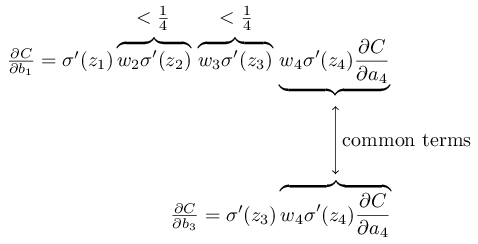
\includegraphics[width=0.9\textwidth]{images/tikz39.png}
\end{center}

\noindent 这两个表达式共享许多项. 但梯度 $\partial C / \partial b_1$ 多包含了两个形如 $w_j \sigma'(z_j)$ 的项. 正如我们所看到的，这样的项通常大小小于 $1/4$. 因此梯度 $\partial C / \partial b_1$ 通常会比 $\partial C / \partial b_3$ 小 $16$ 倍（或更多）. 这就是梯度消失问题的本质根源.

当然，这是一个非正式的论证，而不是梯度消失问题一定会发生的严格证明. 存在几种可能的例外情况. 特别地，我们可能会想权重 $w_j$ 在训练过程中是否会增大. 如果它们增大了，那么乘积中的项 $w_j \sigma'(z_j)$ 可能不再满足 $|w_j \sigma'(z_j)| < 1/4$. 确实，如果这些项变得足够大——大于 $1$——那么我们将不再有梯度消失问题. 相反，当我们反向穿过各层时，梯度实际上会指数级增长. 我们将遇到的不是梯度消失问题，而是梯度爆炸\label{term:66}问题.\textbf{梯度爆炸问题：} 让我们看一个梯度爆炸发生的具体例子. 这个例子有些人为构造：我将以恰到好处的方式固定网络中的参数，以确保我们得到梯度爆炸. 但即使这个例子是人为构造的，它的优点在于牢固地确立了梯度爆炸不仅仅是一种假设的可能性，它们确实可以发生.

得到梯度爆炸需要两个步骤. 首先，我们选择网络中所有较大的权重，比如 $w_1 = w_2 = w_3 = w_4 = 100$. 其次，我们选择偏置使得 $\sigma'(z_j)$ 项不会太小. 这实际上很容易做到：我们只需要选择偏置使得每个神经元的加权输入为 $z_j = 0$（从而 $\sigma'(z_j) = 1/4$）. 例如，我们想要 $z_1 = w_1 a_0 + b_1 = 0$. 我们可以通过设置 $b_1 = -100 * a_0$ 来实现这一点. 我们可以用同样的思路来选择其他偏置. 当我们这样做时，我们看到所有项 $w_j \sigma'(z_j)$ 都等于 $100 * \frac{1}{4} = 25$. 有了这些选择，我们就得到了梯度爆炸.\textbf{不稳定的梯度问题：} 这里根本的问题与其说是梯度消失问题或梯度爆炸问题，不如说是早期层中的梯度是所有后面层中项的乘积. 当有很多层时，这本质上是一种不稳定的情况. 所有层能够以接近相同的速度学习的唯一方式是所有这些项的乘积接近相互平衡. 如果没有某种机制或内在原因使得这种平衡发生，它极不可能仅仅靠偶然发生. 简而言之，这里真正的问题是神经网络遭受\emph{不稳定的梯度问题}（unstable gradient problem）\label{term:65}. 因此，如果我们使用标准的基于梯度的学习技术，网络中不同的层将倾向于以极其不同的速度学习.

\begin{exerciseBox}{练习}

\begin{itemize}

\item 在我们对梯度消失问题的讨论中，我们利用了 $|\sigma'(z)| < 1/4$ 这一事实. 假设我们使用一个不同的激活函数，其导数可能大得多. 这能帮助我们避免不稳定的梯度\label{term:67}问题吗？

\end{itemize}

\textbf{梯度消失问题的普遍性：} 我们已经看到，在深度网络的早期层中梯度要么消失要么爆炸. 事实上，当使用 S 型神经元时，梯度通常会消失. 要理解原因，再次考虑表达式 $|w \sigma'(z)|$. 为了避免梯度消失问题，我们需要 $|w \sigma'(z)| \geq 1$. 你可能认为如果 $w$ 非常大，这很容易发生. 然而，这比看起来要困难. 原因是 $\sigma'(z)$ 项也依赖于 $w$：$\sigma'(z) = \sigma'(wa +b)$，其中 $a$ 是输入激活值. 所以当我们使 $w$ 变大时，我们需要注意不要同时使 $\sigma'(wa+b)$ 变小. 事实证明这是一个相当大的约束. 原因是当我们使 $w$ 变大时，我们倾向于使 $wa+b$ 非常大. 看着 $\sigma'$ 的图像，你可以看到这把我们带到了 $\sigma'$ 函数的``两翼''，在那里它取非常小的值. 避免这种情况的唯一方法是输入激活值落在一个相当窄的值范围内（这个定性解释在下面的第一个习题中被定量化）. 有时这会碰巧发生. 但更常见的是，它不会发生. 所以在一般情况下我们有梯度消失.

\end{exerciseBox}

\begin{exerciseBox}{习题}

\begin{itemize}

\item
考虑乘积 $|w \sigma'(wa+b)|$. 假设 $|w \sigma'(wa+b)| \geq 1$.(1) 论证这只有在 $|w| \geq 4$ 时才可能发生.(2) 假设 $|w| \geq 4$，考虑满足 $|w \sigma'(wa+b)| \geq 1$ 的输入激活值 $a$ 的集合. 证明满足该约束的 $a$ 的集合所覆盖的区间宽度不超过

\begin{equation}
\frac{2}{|w|} \ln\left( \frac{|w|(1+\sqrt{1-4/|w|})}{2}-1\right).
\tag{123}
\end{equation}

(3) 用数值方法证明上述界定区间宽度的表达式在 $|w| \approx 6.9$ 处最大，此时它取值 $\approx 0.45$. 因此，即使一切都完美地对齐，我们仍然只有一个相当窄的输入激活值范围可以避免梯度消失问题.

\item \textbf{恒等神经元：} 考虑一个神经元，它有一个输入 $x$，对应的权重 $w_1$，一个偏置 $b$，以及输出上的权重 $w_2$. 证明通过适当地选择权重和偏置，我们可以确保对于 $x \in [0, 1]$ 有 $w_2 \sigma(w_1 x+b) \approx x$. 这样的神经元因此可以被用作一种恒等神经元，即一个输出与其输入相同（至多相差一个权重因子的缩放）的神经元.\emph{提示：把 $x = 1/2+\Delta$ 重写，假设 $w_1$ 很小，并对 $w_1 \Delta$ 使用泰勒级数展开，这些都会有所帮助.}

\end{itemize}

\end{exerciseBox}
\sectionTitle{更复杂网络中不稳定的梯度}{更复杂网络中不稳定的梯度}

我们一直在研究玩具网络，每个隐藏层只有一个神经元. 那么更复杂的深度网络呢，每个隐藏层中有许多神经元？

\begin{center}
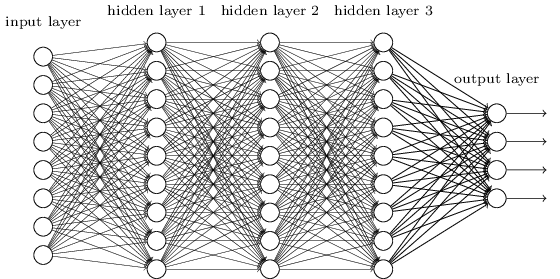
\includegraphics[width=0.9\textwidth]{images/tikz40.png}
\end{center}

事实上，这类网络中会出现大致相同的行为. 在之前关于反向传播的章节中，我们看到 $L$ 层网络中第 $l$ 层的梯度由下式给出：

\begin{equation}
\delta^l = \Sigma'(z^l) (w^{l+1})^T \Sigma'(z^{l+1}) (w^{l+2})^T \ldots \Sigma'(z^L) \nabla_a C
\tag{124}
\end{equation}

\noindent 这里，$\Sigma'(z^l)$ 是一个对角矩阵，其对角线元素是第 $l$ 层加权输入的 $\sigma'(z)$ 值. $w^l$ 是不同层的权重矩阵. 而 $\nabla_a C$ 是 $C$ 关于输出激活值的偏导数向量.

这比单神经元情形下的表达式要复杂得多. 不过，如果你仔细观察，其基本形式非常相似，包含许多形如 $(w^j)^T \Sigma'(z^j)$ 的项对. 更重要的是，矩阵 $\Sigma'(z^j)$ 的对角线元素很小，没有一个大于 $\frac{1}{4}$. 只要权重矩阵 $w^j$ 不太大，每个额外的项 $(w^j)^T \Sigma'(z^l)$ 都会倾向于使梯度向量变小，从而导致梯度消失. 更一般地，乘积中大量的项倾向于导致不稳定的梯度，正如我们之前的例子那样. 在实践中，经验上通常发现，在 S 型网络中，梯度在较早的层中会以指数速度迅速消失. 结果，这些层中的学习会减慢. 这种减慢不仅仅是偶然的或不方便的事情：它是我们采用的学习方法的根本后果.
\sectionTitle{深度学习的其他障碍}{深度学习的其他障碍}

在本章中，我们关注了梯度消失——更一般地说，不稳定的梯度——作为深度学习的一个障碍. 事实上，不稳定的梯度只是深度学习的一个障碍，尽管它是一个重要的根本性障碍. 许多正在进行的研究旨在更好地理解训练深度网络时可能出现的挑战. 我不会在这里全面总结这些工作，而只是想简要提及几篇论文，让你感受一下人们正在提出的一些问题.

作为第一个例子，2010 年 Glorot 和 Bengio*\footnote{Understanding the difficulty of training deep feedforward neural networks, by Xavier Glorot and Yoshua Bengio (2010). See also the earlier discussion of the use of sigmoids in Efficient BackProp, by Yann LeCun, Léon Bottou, Genevieve Orr and Klaus-Robert Müller (1998).} 发现了证据，表明使用 S 型激活函数可能会导致训练深度网络时出现问题. 特别地，他们发现证据表明，使用 S 型函数会导致最终隐藏层中的激活值在训练早期就饱和在 $0$ 附近，从而大幅减慢学习速度. 他们提出了一些替代的激活函数，这些函数似乎不太受这个饱和问题的影响.

作为第二个例子，2013 年 Sutskever、Martens、Dahl 和 Hinton*\footnote{On the importance of initialization and momentum in deep learning, by Ilya Sutskever, James Martens, George Dahl and Geoffrey Hinton (2013).} 研究了随机权重初始化和基于动量的随机梯度下降中的动量日程对深度学习的影响. 在这两种情况下，做出好的选择对训练深度网络的能力产生了实质性的差异.

这些例子表明，``是什么让深度网络难以训练？'' 是一个复杂的问题. 在本章中，我们关注了与深度网络中基于梯度的学习相关的不稳定性. 最后两段中的结果表明，激活函数的选择、权重的初始化方式，甚至梯度下降学习的实现细节也发挥着作用. 当然，网络结构和其他超参数的选择也很重要. 因此，许多因素都可能在使深度网络难以训练中发挥作用，而理解所有这些因素仍然是一个正在进行的研究课题. 这一切似乎相当令人沮丧和悲观. 但好消息是，在下一章中我们将扭转局面，并开发几种深度学习方法，这些方法在一定程度上设法克服或绕开所有这些挑战.
